\question Determine whether the graphs \(G_1\) and \(G_2\)
are bipartite. If a graph is bipartite, then redraw it
indicating the partite sets; if not, then give an 
explanation as to why the graph is not bipartite.

\begin{center}
  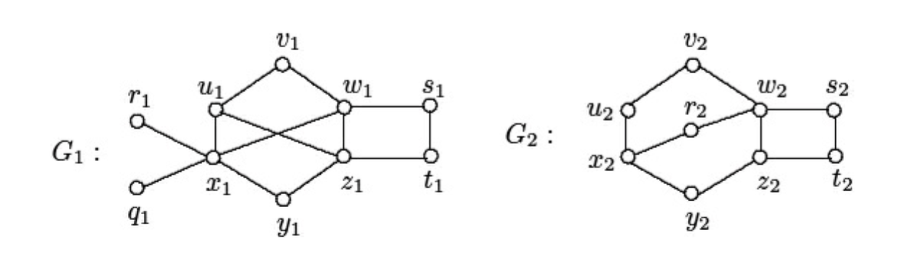
\includegraphics[width=0.69\textwidth]{figures/p1-graphs}
\end{center}

\begin{solution}
  Note that checking for bipartite-ness of a graph can be
  formulated as a graph coloring problem. Namely, we color the
  graph such that adjacent vertices must always have different
  colors. We will use orange and blue to show this.

  \(G_1\) is bipartite and the vertices can be split into 
  \(A = \{x_1, v_1, z_1, s_1\} \) and \(B = \{r_1, q_1, u_1,
  y_1, w_1, t_1\}\).
  \begin{center}
    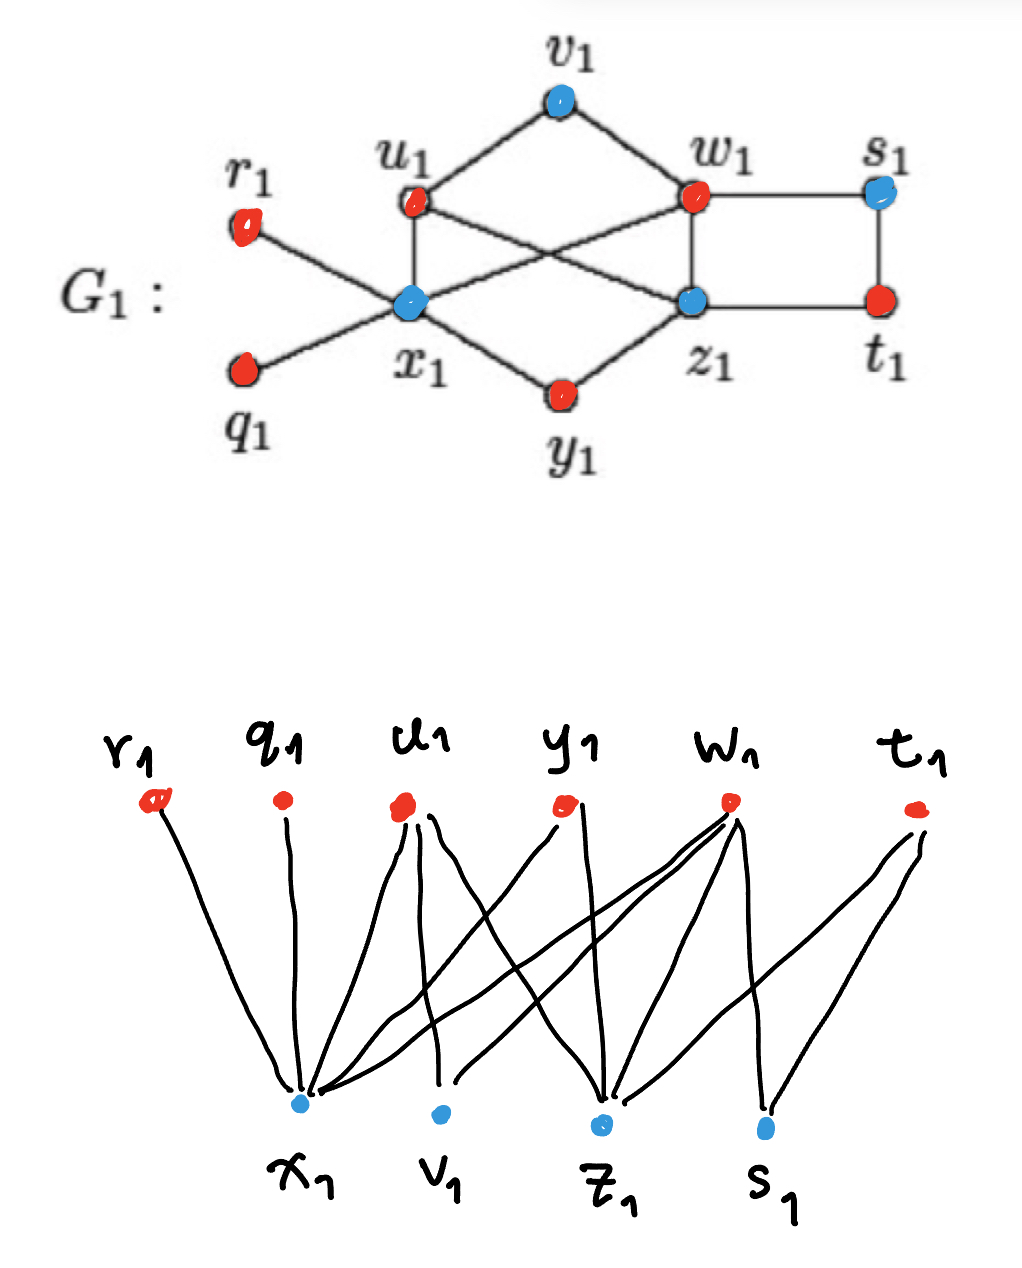
\includegraphics[width=0.3\textwidth]{figures/p1-g1}
  \end{center}

  On the other hand, \(G_2\) is not bipartite. Notice that in the
  diagram below that the cycle \(x_2-u_2-v_2-w_2-z_2-y_2\) has 6
  vertices, so we are able to color them with 2 colors. However,
  notice also that \(x_2\) and \(w_2\) will always have different
  colors. So, it is impossible to paint the path \(x_2-r_2-w_2\)
  with only 2 colors since \(r_2\) would already be adjacent to
  2 different colors already.
  \begin{center}
    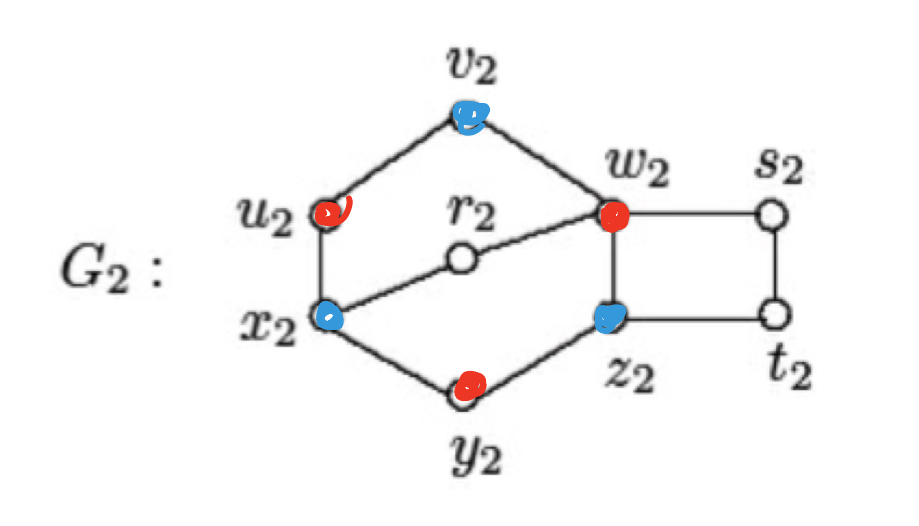
\includegraphics[width=0.3\textwidth]{figures/p1-g2}
  \end{center}
\end{solution}
